\chapter{Numerical Solution of Flow Equations}
\label{chapter-three}

\section{Fully-Coupled Point Implicit Method}

The governing equations presented in \erefs{species-cons}{tot-energy-cons} can
be recast in vector form as
%------------------------------------------------------------------------------%
\begin{equation}
	\label{inv_flux_vec}
	\frac{\partial \mathbf{U}}{\partial t}
	+ \nabla\cdot \mathbf{F} = \mathbf{W}
\end{equation}
%------------------------------------------------------------------------------%
 or, in semi-discrete form,
%------------------------------------------------------------------------------%
\begin{equation}
	\label{inv_flux_fv}
	\frac{\partial \mathbf{U}}{\partial t}
	 + \frac{1}{V}\sum\limits_{f}(\mathbf{F}\cdot\mathbf{S})^f = \mathbf{W}
 \end{equation}
%------------------------------------------------------------------------------%
summing over all faces, $f$, in the domain, where V is the cell volume, 
$\mathbf{W}$ is the chemical source term vector, and $\mathbf{S}$ is the face
outward normal vector.  The vectors of conserved variables and fluxes are:
%------------------------------------------------------------------------------%
\begin{equation}
	\begin{matrix}
	\mathbf{U}=\begin{pmatrix}
   		\rho_1\\
		\vdots \\
		\rho_{ns} \\
		\rho u \\
		\rho v \\
		\rho w \\
		\rho E \\
	\end{pmatrix},      &
 	\mathbf{F} = \begin{pmatrix}
		\rho_1  \overline{U} \\
		\vdots \\
		\rho_{ns} \overline{U} \\
		\rho u \overline{U} + p s_x\\
		\rho u \overline{U} + p s_y\\
		\rho u \overline{U} + p s_z\\
		(\rho E + p) \overline{U} \\
	\end{pmatrix}
	\end{matrix}
 \end{equation}
%------------------------------------------------------------------------------%
where $\overline{U}$ is the outward pointing normal velocity, $E$ is
the total energy of the mixture per unit mass as defined in
\eref{tot-energy-def}, and $e_s$ is the internal energy of species $s$ as
defined in \eref{int-energy-def}.  By using the Roe FDS scheme,
%------------------------------------------------------------------------------%
\begin{equation}
	\begin{matrix}
		\mathbf{F}^{n+1} \approx \mathbf{F}^n+\frac{\partial \mathbf{F}}{\partial \mathbf{U}}\delta\mathbf{U}^n \\
		\\
		\mathbf{W}^{n+1} \approx \mathbf{W}^n+\frac{\partial \mathbf{W}}{\partial \mathbf{U}}\delta\mathbf{U}^n \\
	\end{matrix}
\end{equation}
%------------------------------------------------------------------------------%
where $\delta\mathbf{U}^n = \mathbf{U}^{n+1}- \mathbf{U}^{n}$.  By using an implicit time integration, the implicit scheme becomes:
%------------------------------------------------------------------------------%
\begin{equation}
	\frac{\mathbf{\delta U}^n}{\Delta t}+\frac{1}{V}\sum\limits_{f}(\frac{\partial \mathbf{F}^f}{\partial \mathbf{U^L}}\delta\mathbf{U}^L
	+\frac{\partial \mathbf{F}^f}{\partial \mathbf{U^R}}\delta\mathbf{U}^R)^n \mathbf{S}^f
	- \frac{\partial \mathbf{W}}{\partial \mathbf{U}}\delta\mathbf{U}^n
	= -\frac{1}{V}\sum\limits_{f}(\mathbf{F}^f\cdot\mathbf{S}^f)^n + \mathbf{W}^n
\end {equation}
%
or, put more simply:
%
\begin{equation}
	A\delta\mathbf{U}^n = \mathbf{b}
\end{equation}
%------------------------------------------------------------------------------%
where $A$ is the Jacobian matrix of the fully coupled system, and $\mathbf{b}$
is the residual vector.  For a point implicit relaxation scheme, the Jacobian
matrix can be split into its diagonal and off-diagonal elements, with the latter
moved to the RHS:
%------------------------------------------------------------------------------%
\begin{equation}
\label{decomp_jac}
	A=O+D
\end{equation}
%------------------------------------------------------------------------------%
Each matrix element is a square $(ns+4)\times(ns+4)$ matrix.  One method of
solving this system is a Red-Black Gauss-Seidel scheme\cite{red-black}, where
matrix coefficients with even indices are updated first and, subsequently, the
coefficients with odd indices are updated.  This red-black ordering enables
better vectorization in solving the linear system.  The computational work for
the Gauss-Seidel scheme is dominated by matrix-vector multiplications of
elements of $O$ with $\delta\mathbf{U}$, which are $O(N^2)$ operations, where
$N=ns+4$.  In the next section, it is shown that decoupling the system reduces
these matrix-vector multiplications to $O(N^2 + M)$ operations, where $N=ns$ and
$M=ns$.

\section{Decoupled Point Implicit Method}

If the species mass equations are replaced by a single mixture mass equation,
the mixture equations can be separated from the species mass
equations and the conserved variables become
%------------------------------------------------------------------------------%
\begin{equation}
	\begin{matrix}
		\mathbf{U}'=\begin{pmatrix}
			\rho \\
			\rho u \\
			\rho v \\
			\rho w \\
			\rho E
		\end{pmatrix} &
		\mathbf{\hat{U}}=\begin{pmatrix}
			\rho_1 \\
			\vdots \\
			\rho_{ns}
		\end{pmatrix}
	\end{matrix}
  \label{dc-variables}
\end{equation}
%------------------------------------------------------------------------------%
Solving the flux vector is performed in two sequential steps.  The mixture
fluxes are first solved as
%------------------------------------------------------------------------------%
\begin{equation}
  \frac{\partial \mathbf{{U}'}}{\partial t} +
  \frac{1}{V}\sum\limits_{f}(\mathbf{F}'\cdot\mathbf{S})^f = 0
\end{equation}
%------------------------------------------------------------------------------%
followed by the species fluxes as
%------------------------------------------------------------------------------%
\begin{equation}
  \frac{\partial \mathbf{\hat{U}}}{\partial t} +
  \frac{1}{V}\sum\limits_{f}(\mathbf{\hat{F}}\cdot\mathbf{S})^f =
  \mathbf{\hat{W}}
\end{equation}
%------------------------------------------------------------------------------%
Point relaxation uses Red-Black Gauss-Seidel to update the conserved
variables in $\mathbf{U}'$ and all associated auxiliary variables, such as
temperature, pressure, speed of sound, etc.  This is done by holding the
thermo-chemical state constant, and will always result in the relaxation of a
five-equation system.  This does trade an implicit relationship between the mixture
and species equations for an explicit one; thus, this decoupling can have an
impact on the stability of the scheme, especially due to the non-linearity of
the chemical source term\cite{park}.
 
The solution of the species mass equations takes a different form.  Based on the
work of Candler et al.\cite{candler}, the decoupled variables can be rewritten
in terms of mass fraction, as follows:
%------------------------------------------------------------------------------%
\begin{equation}
  \delta \mathbf{\hat{U}}^n =
  \rho^{n+1}\mathbf{\hat{V}}^{n+1}-\rho^n\mathbf{\hat{V}}^n = \rho^{n+1} \delta
  \mathbf{\hat{V}}^n + \mathbf{\hat{V}}^n \delta \rho^n 
\end{equation}
%------------------------------------------------------------------------------%
where $\mathbf{\hat{V}}=(c_1,\hdots,c_{ns})^T$, and $c_s=\rho_s/\rho$ the mass
fraction of species $s$.  While the derivation of the species mass equations is
different for the Roe FDS scheme from that of Steger-Warming proposed by Candler
et al.\cite{candler}, the final result takes a similar form: 
%------------------------------------------------------------------------------%
\begin{gather}
  \hat{F}_{\rho_s} = c_s F'_\rho+(c_s^L-\tilde{c}_s)\rho^L\lambda^+
  + (c_s^R-\tilde{c}_s)\rho^R\lambda^-
  \label{dc_flux}
\end{gather}
%------------------------------------------------------------------------------%
where $F_\rho'$ is the total mass flux computed previously using all
$\mathbf{U}'$ variables, and $\tilde{}$ denotes a Roe-averaged quantity.
Likewise, linearizing the species mass fluxes with respect to the
$\mathbf{\hat{V}}$ variables yields
%------------------------------------------------------------------------------%
\begin{align} 
  \mathbf{\hat{F}}^{n+1} &= \mathbf{\hat{F}}^n +\frac{\partial
  \mathbf{\hat{F}}}{\partial \mathbf{\hat{V}}^L}\delta \mathbf{\hat{V}}^L
  +\frac{\partial \mathbf{\hat{F}}}{\partial \mathbf{\hat{V}}^R}\delta
  \mathbf{\hat{V}}^R \\ \frac{\partial \mathbf{\hat{F}}}{\partial
  \mathbf{\hat{V}}^L} &= wF_\rho+(1-w)\rho^L\lambda^+ - w\rho^R\lambda^- \\
  \frac{\partial \mathbf{\hat{F}}}{\partial \mathbf{\hat{V}}^R} &=
  (1-w)F_\rho+(w-1)\rho^L\lambda^+ + w\rho^R\lambda^-
  \label{d_last}
\end{align}
%------------------------------------------------------------------------------%
A full derivation of \erefs{dc_flux}{d_last}, along with the
definition of $w$, is included in Appendix A.  The chemical source term is
linearized in the same manner as the fully coupled scheme; however, the updated
$\mathbf{U}'$ variables are used to evaluate the Jacobian, and the chain rule is
applied to linearize $\mathbf{\hat{W}}$ with respect to the species mass
fractions:
%------------------------------------------------------------------------------%
\begin{equation}
  \mathbf{\hat{W}}^{n+1} = \mathbf{\hat{W}}^n+\frac{\partial
  \mathbf{\hat{W}}}{\partial \mathbf{U}}\bigg|_{\mathbf{U}'} \frac{\partial
  \mathbf{U}}{\partial \mathbf{\hat{V}}} 
\end{equation}
%------------------------------------------------------------------------------%
For simplicity of notation, we define
%------------------------------------------------------------------------------%
\begin{equation}
  C = \frac{\partial \mathbf{\hat{W}}}{\partial
  \mathbf{U}}\bigg|_{\mathbf{U}'} \frac{\partial \mathbf{U}}{\partial
  \mathbf{\hat{V}}}
\end{equation}
%------------------------------------------------------------------------------%
The decoupled system to be solved becomes:
%------------------------------------------------------------------------------%
\begin{gather} 
  \begin{split}
    \rho^{n+1}&\frac{\mathbf{\delta \hat{V}}^n}{\Delta t}
    +\frac{1}{V}\sum\limits_{f}(\frac{\partial \mathbf{\hat{F}}^f}{\partial
    \mathbf{\hat{V}}^L}\delta	\mathbf{\hat{V}}^L
    +\frac{\partial \mathbf{\hat{F}}^f}{\partial \mathbf{\hat{V}}^R}\delta
    \mathbf{\hat{V}}^R)^{n, n+1}\mathbf{S}^f - C^{n, n+1}\delta\mathbf{V}^n \\
    &= -\frac{1}{V}\sum\limits_{f}(\mathbf{\hat{F}}^{n,n+1}\cdot\mathbf{S})^f +
    \mathbf{W}^{n, n+1} -\mathbf{\hat{V}}^n\frac{\delta \rho^n}{\Delta t} -
    R_\rho
  \end{split} \\ 
  R_\rho = -\frac{1}{V}\sum\limits_{f}{\sum\limits_{s}
  {(\hat{F}_{\rho_s}^{n,n+1}\cdot\mathbf{S})}}
\end{gather}
%------------------------------------------------------------------------------%
where $R_\rho$ is included to preserve the constraint that the mass fractions
sum to unity, i.e., $\sum\limits_{s}{c_s}=1$, $\sum\limits_{s}{\delta
c_s}=0$.

\section{Predicted Cost and Memory Savings of the Decoupled Implicit Problem}

In decoupling the species equations, the most significant savings comes from the
source term linearization being purely node-based\cite{gnoffo-tp}.  Solving the
mean flow equations is conducted in the same manner as the fully coupled system.
All entries in the Jacobian $A_m$ are linearizations of the mixture equation
fluxes, which results in $5\times5$ matrices. All entries in the Jacobian $A_d$
are linearizations of the species mass fluxes, which results in $ns \times ns$
matrices.  Because there is no interdependence of species, except through the
chemical source term, all contributions due to linearizing the convective flux
are purely diagonal $ns \times ns$ matrices.  Via \eref{decomp_jac}, we
decompose $A_d$ into its diagonal and off-diagonal elements, resulting in the
following linear system:
%------------------------------------------------------------------------------%
\begin{equation}
  \label{dc_sys} 
  \begin{pmatrix} 
    \Box & & & & \\ & \ddots & & & \\ & & \Box \\ & & & \ddots & \\ & & & & \Box
  \end{pmatrix}
  \begin{pmatrix}
    \delta \mathbf{\hat{V}}_1 \\ \vdots \\ \delta \mathbf{\hat{V}}_i \\ 
    \vdots \\ \delta \mathbf{\hat{V}}_{nodes}
  \end{pmatrix}
  =
  \begin{pmatrix}
    \hat{b}_1 \\ \vdots \\ \hat{b}_i \\ \vdots \\ \hat{b}_{nodes} 
  \end{pmatrix}
  -
  \begin{pmatrix}
    (\sum_{j=1}^{N_{nb}}{[\diagdown] \delta\mathbf{\hat{V}}_{j}})_1 \\ \vdots \\
    (\sum_{j=1}^{N_{nb}}{[\diagdown] \delta\mathbf{\hat{V}}_{j}})_i \\ \vdots \\
    (\sum_{j=1}^{N_{nb}}{[\diagdown] \delta\mathbf{\hat{V}}_{j}})_{nodes}
  \end{pmatrix} 
\end{equation} 
%------------------------------------------------------------------------------%
where $\Box$ represents a dense $ns \times ns$ matrix, $[\diagdown]$ represents
a diagonal matrix, and $\delta \mathbf{\hat{V}}_j$  is the decoupled variable
update on the node $j$ that neighbors node $i$, where $N_{nb}$ is the number of
nodes neighboring node $i$.  Thus, the non-zero entries in the off-diagonal
matrix can be reduced from diagonal matrices to vectors.  This results in
significant savings in both computational cost and memory, as the only quadratic
operation left in solving the implicit system is dealing with the diagonal
entries in the Jacobian.  Because the off-diagonal entries significantly
outnumber the diagonal entries, we can expect nearly linear scaling in cost with
the number of species.  If compressed row storage\cite{George} is used to
only store non-zero off-diagonal entries, the relative memory savings in the
limit of a large number of species for the Jacobian is given by
%------------------------------------------------------------------------------%
\begin{equation}
  \label{mem_req_eq}
  \begin{split} 
    Relative\ Memory\ Cost &=
    \frac{size(A_d)}{size(A)} \\ &= \lim_{ns\to\infty}
    \frac{(ns^2+5^2)(N_{nodes})+(ns+5^2)(N_{nz})}{(ns+4)^2(N_{nodes}+N_{nz})} \\
    &= \frac{N_{nodes}}{N_{nodes} + N_{nz}}
  \end{split}
\end{equation}
%------------------------------------------------------------------------------%
where $N_{nodes}$ is the number of nodes, and $N_{nz}$ is the number of non-zero
off-diagonal entries stored using compressed row storage. For a structured grid,
each node has six neighbors in 3D, i.e., $N_{nz} = 6N_{nodes}$; therefore, we can
expect the Jacobian memory required to decrease by a factor of seven using this
decoupled scheme. Interestingly, for a grid that is not purely hexahedra,
$N_{nz} > 6N_{nodes}$; thus, this decoupled scheme provides higher relative
memory savings on unstructured grids than structured grids when using compressed
row storage.

\section{5 km/s Flow over Cylinder}

Both the proposed decoupled scheme and the traditional, fully coupled approach
have been implemented using FUN3D\cite{FUN3D}.  Demonstrating the improved
efficiency in cost and memory required to utilize the decoupled scheme, and that
both the fully coupled and decoupled approaches converge to the same result, a
grid convergence study was conducted on a simple cylinder geometry (radius 0.5
m).  Due to the presence of strong shocks in blunt body flows, it was
advantageous to generate structured-type grids to preserve grid alignment with
the bow shock. A 50$\times$50, 100$\times$100, and 200$\times$200 family
of grids were adapted using the adaptation capability in FUN3D\cite{adaptation}
to produce shock-aligned grids. These grids serve as a surrogate for conducting
a grid convergence study, in that differences observed between the decoupled and
fully coupled schemes decrease as the average mesh spacing decreases.  These
grids are unstructured, consisting totally of hexahedra elements with a single
cell in the spanwise direction, and the 50$\times$50 grid is shown in Figure
\ref{grid}.  The cell elements of these grids were also subdivided into
tetrahedral elements, and it was verified that there are no issues with a true
unstructured grid topology.  The free stream conditions used were $V_{\infty} =
5000\ m/s$, $\rho_{\infty}=0.001\ kg/m^3$, and $T_\infty = 200\ K$.  Several
chemical kinetics models were used, including a 5-species model with 5
reactions, an 11-species model with 22 reactions, and an 18-species model with
29 reactions.  All cases were run in thermodynamic equilibrium, with a
one-temperature model.

%------------------------------------------------------------------------------%
\begin{figure}[h]
	\centering
  \adjincludegraphics[width=0.8\textwidth,trim={0 4cm 0 4cm},clip]{figures/scitech/grid}
	\caption{50$\times$50 cylinder grid.}
  \label{grid}
\end{figure}
%------------------------------------------------------------------------------%

\subsection{Cylinder - Verification of Implementation}

In order to be valid, the decoupled scheme must yield converged solutions that
are nearly identical to those of the fully coupled system. To quantitatively
assess this, we compare the predicted surface pressure, surface temperature, and
the species composition on the stagnation line for both schemes.  Figure
\ref{pq} shows the predicted quantities on the 100$\times$100 grid, for species
mixture of N, $\text{N}_2$, O, $\text{O}_2$, and NO with five reactions. All
results are indeed nearly identical, with temperature and pressure matching
discretely to eight digits and the species mass fractions on the stagnation line
matching to four digits.  This difference was further reduced on the finest grid
level of 200$\times$200, suggesting that both schemes converge to the same
solution with grid refinement.
%------------------------------------------------------------------------------%
\begin{figure}[h!]
  \captionsetup[subfigure]{position=b}
  \centering
  \subcaptionbox{Surface pressure}{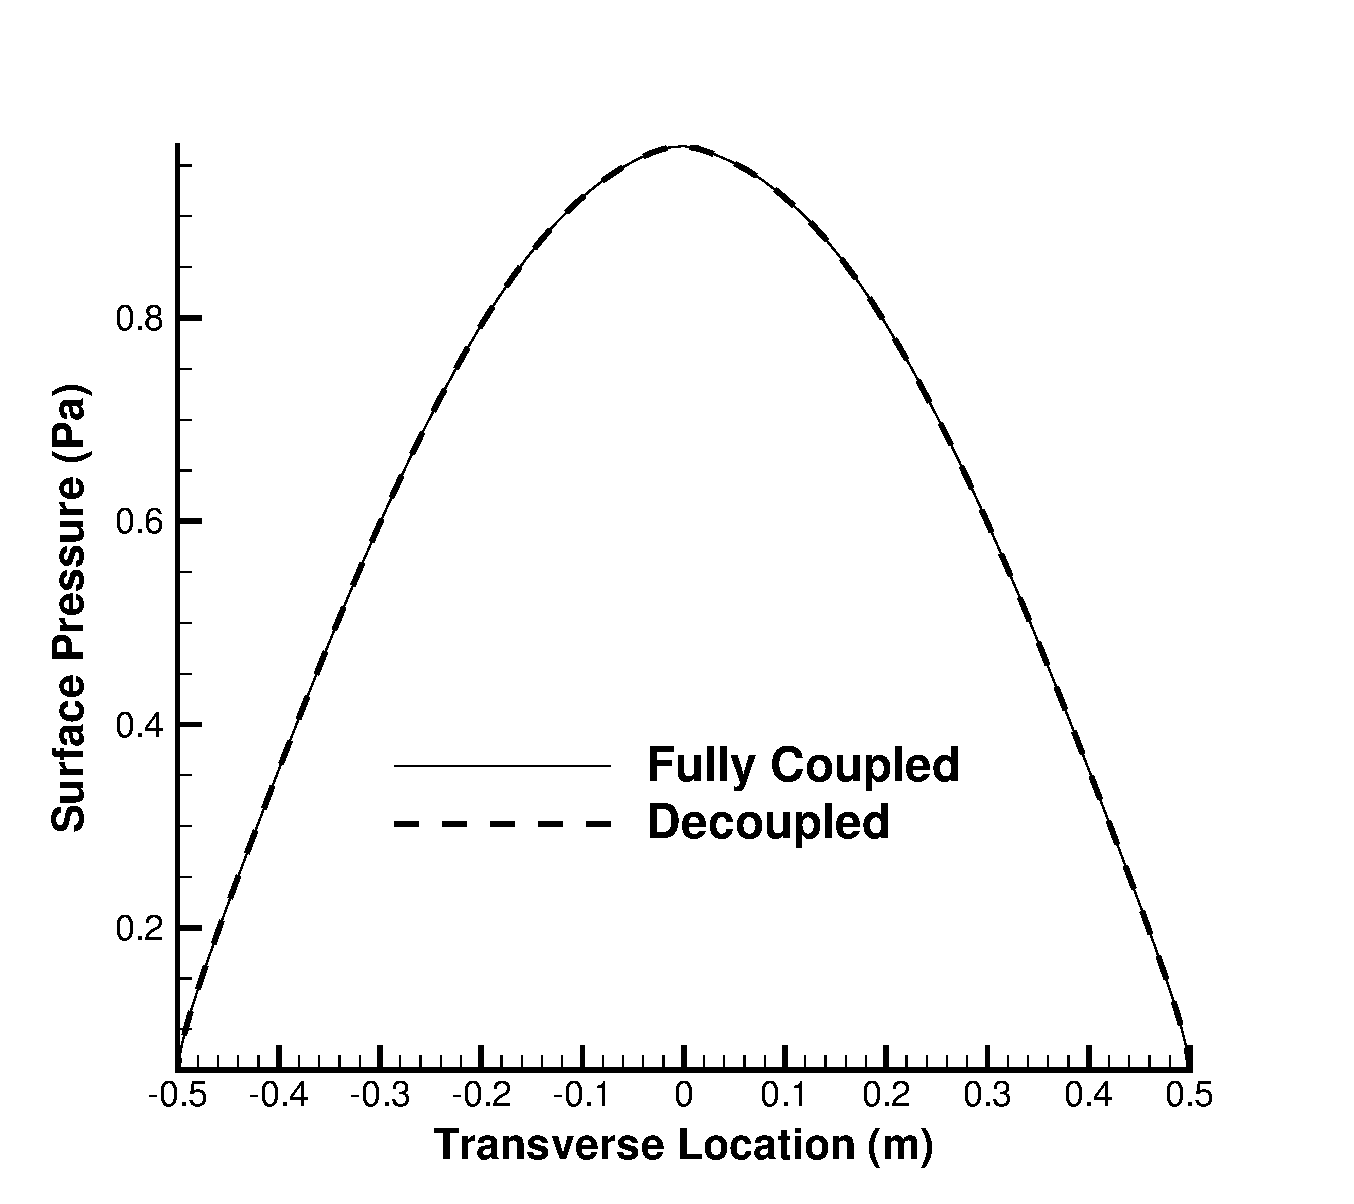
\includegraphics[width=0.3\linewidth]{figures/scitech/surface_pressure}}
  \subcaptionbox{Surface temperature}{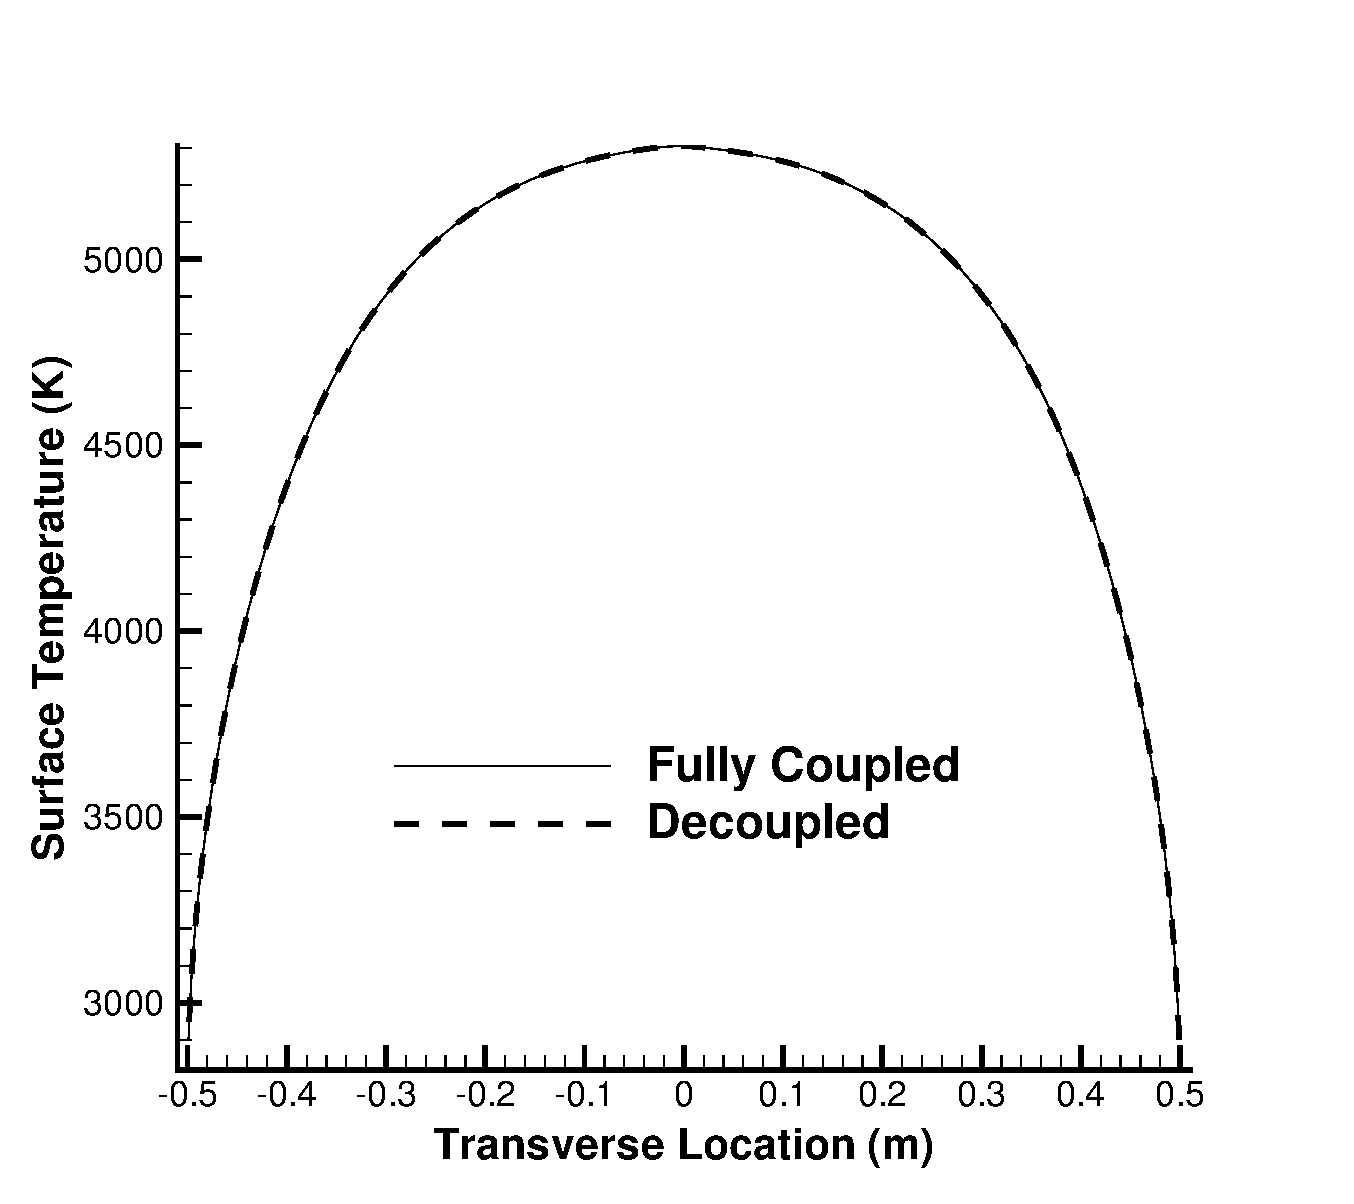
\includegraphics[width=0.3\linewidth]{figures/scitech/surface_temperature}}
  \subcaptionbox{Mass fractions on stagnation line}{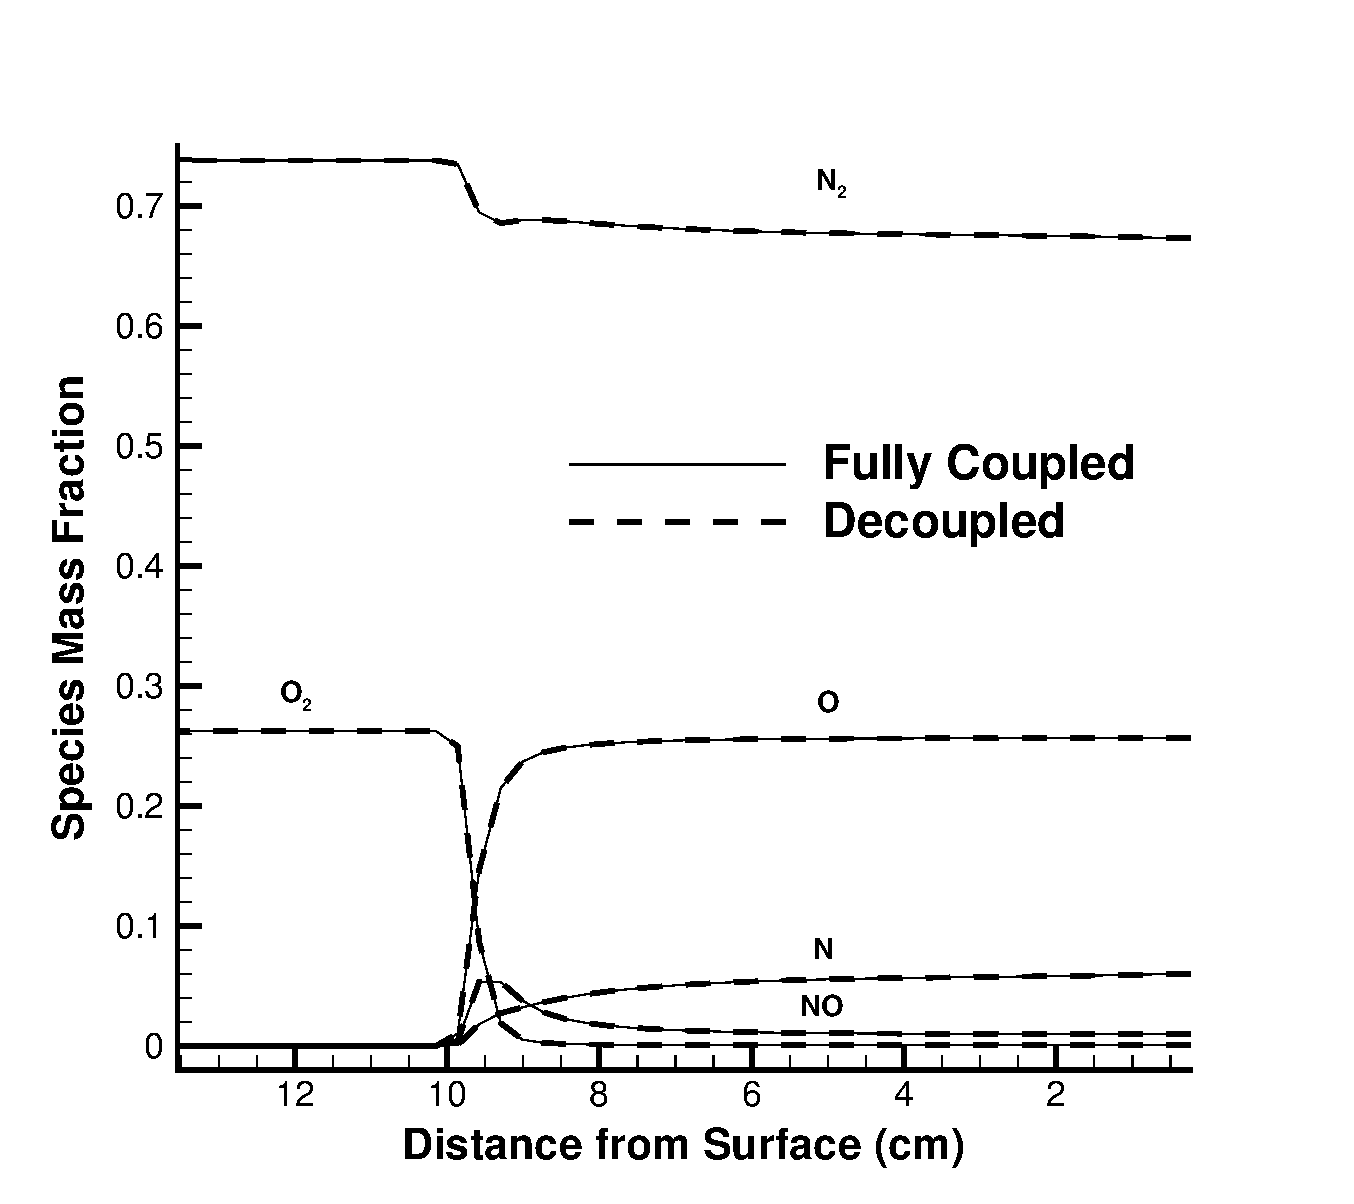
\includegraphics[width=0.32\linewidth]{figures/scitech/stag_line_mf}}
	\caption{Cylinder predicted quantities.}
	\label{pq}
\end{figure}
%------------------------------------------------------------------------------%

\subsection{Cylinder - Memory Cost}

In order to determine the required memory of the decoupled scheme compared
to the fully coupled scheme, a convergence study was conducted using
Valgrind\cite{valgrind} to determine the memory actually allocated by FUN3D for
an increasing number of species.  
Figure \ref{mem_req} shows that the relative memory cost converges asymptotically to
$\sim$1/4, which is nearly twice the predicted value of 1/7.  For the
implementation of FUN3D, this is correct because the off-diagonal entries are
reduced from double to single precision.  Each structured grid node has six
neighboring nodes, with the exception of those at the boundary.  Because each of
these six neighboring nodes yields single precision, off-diagonal Jacobian
elements, 
%------------------------------------------------------------------------------%
\begin{equation} 
  N_{nz} = \frac{6N_{nodes}}{2} = 3N_{nodes}
  \label{f3d_off_diag} 
\end{equation} 
%------------------------------------------------------------------------------%
Substituting \eref{f3d_off_diag} into \eref{mem_req_eq}, the relative memory
cost is:
%------------------------------------------------------------------------------%
\begin{equation} 
  Relative\ Memory\ Cost = 
  \frac{N_{nodes}}{N_{nodes} + N_{nz}} =
  \frac{N_{nodes}}{N_{nodes} + (3N_{nodes})}=\frac{1}{4}
\end{equation}
%------------------------------------------------------------------------------%
%------------------------------------------------------------------------------%
\begin{figure}[h] 
  \begin{center} 
    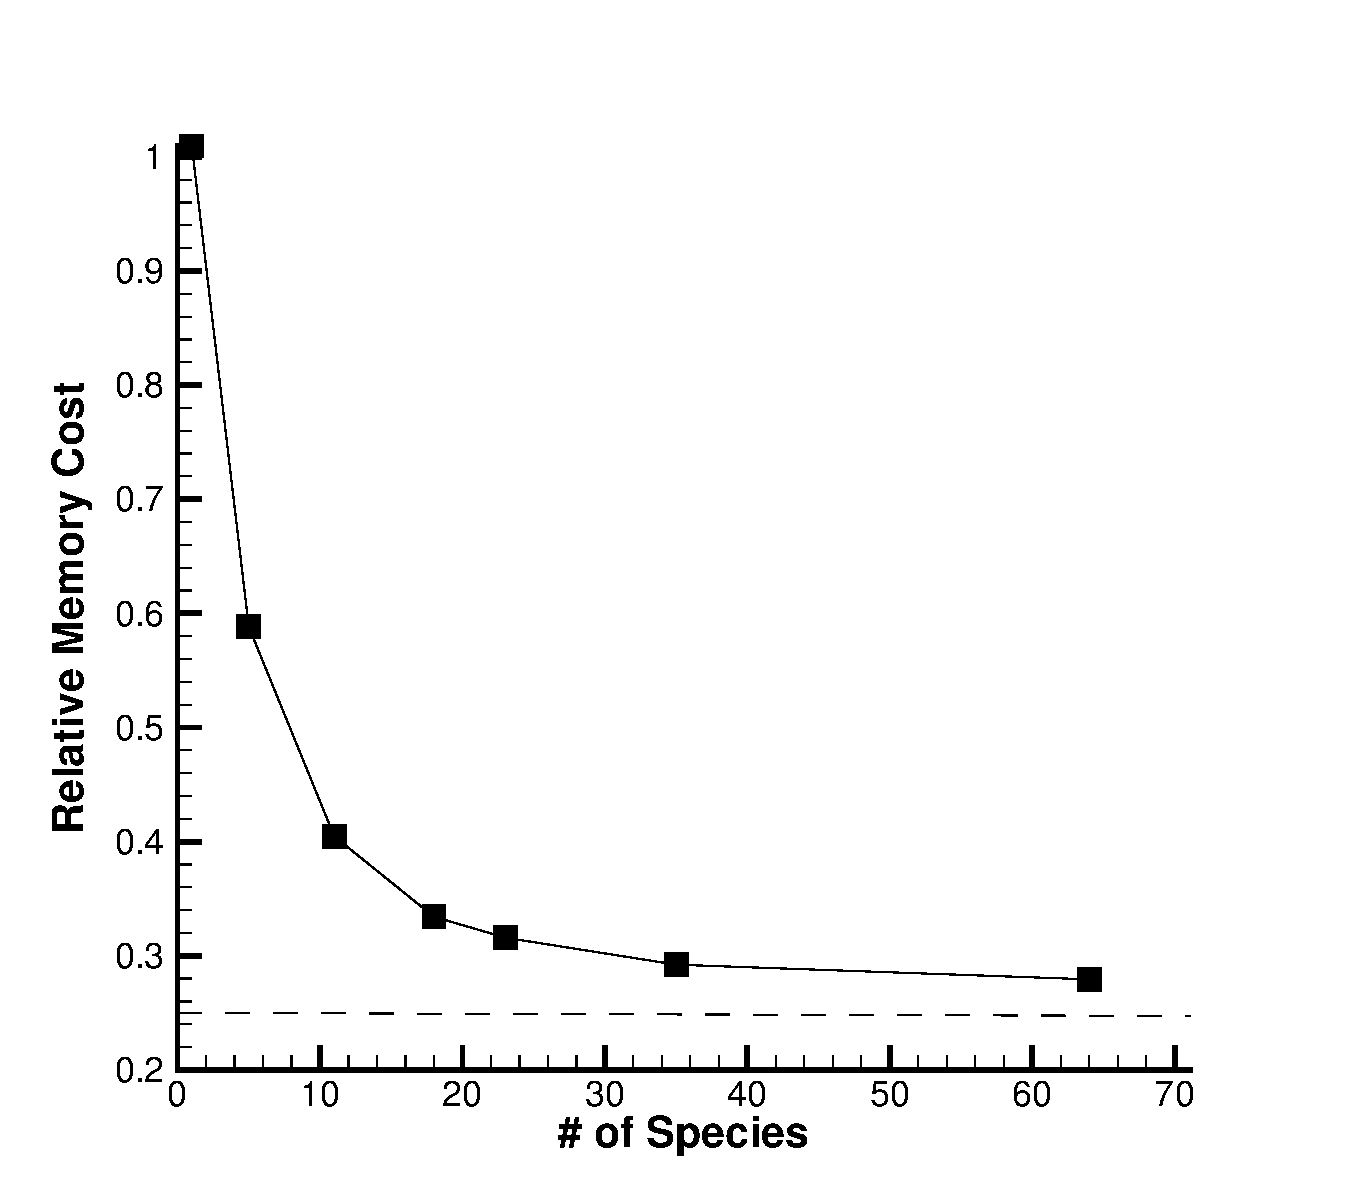
\includegraphics[width=0.45\textwidth]{figures/scitech/mem_req}
    \caption{Memory required convergence study} 
    \vspace{-2em}
    \label{mem_req}
    \end{center} 
\end{figure}
%------------------------------------------------------------------------------%
thus, the relative memory saved by using the decoupled scheme correctly
approaches a factor of 1/4.

\subsection{Cylinder - Computational Cost}

As stated before, the cost of solving the decoupled implicit system should scale
approximately linearly with the number of species, whereas the fully coupled
problem should scale quadratically; thus, the speedup of the implicit solve
should be approximately linear when comparing the decoupled and fully coupled
approaches.  Figure \ref{rel_speedup} shows this to be true for the cylinder test
case, and that the total speedup of the problem is less than that of just
the linear solve.  It is to be expected that the overall gains are not as large
as those for the implicit solve, since there are many other factors that
scale with the number of species, especially calculating the species source term
and its linearization.

%------------------------------------------------------------------------------%
\begin{figure}[h]
  \centering
  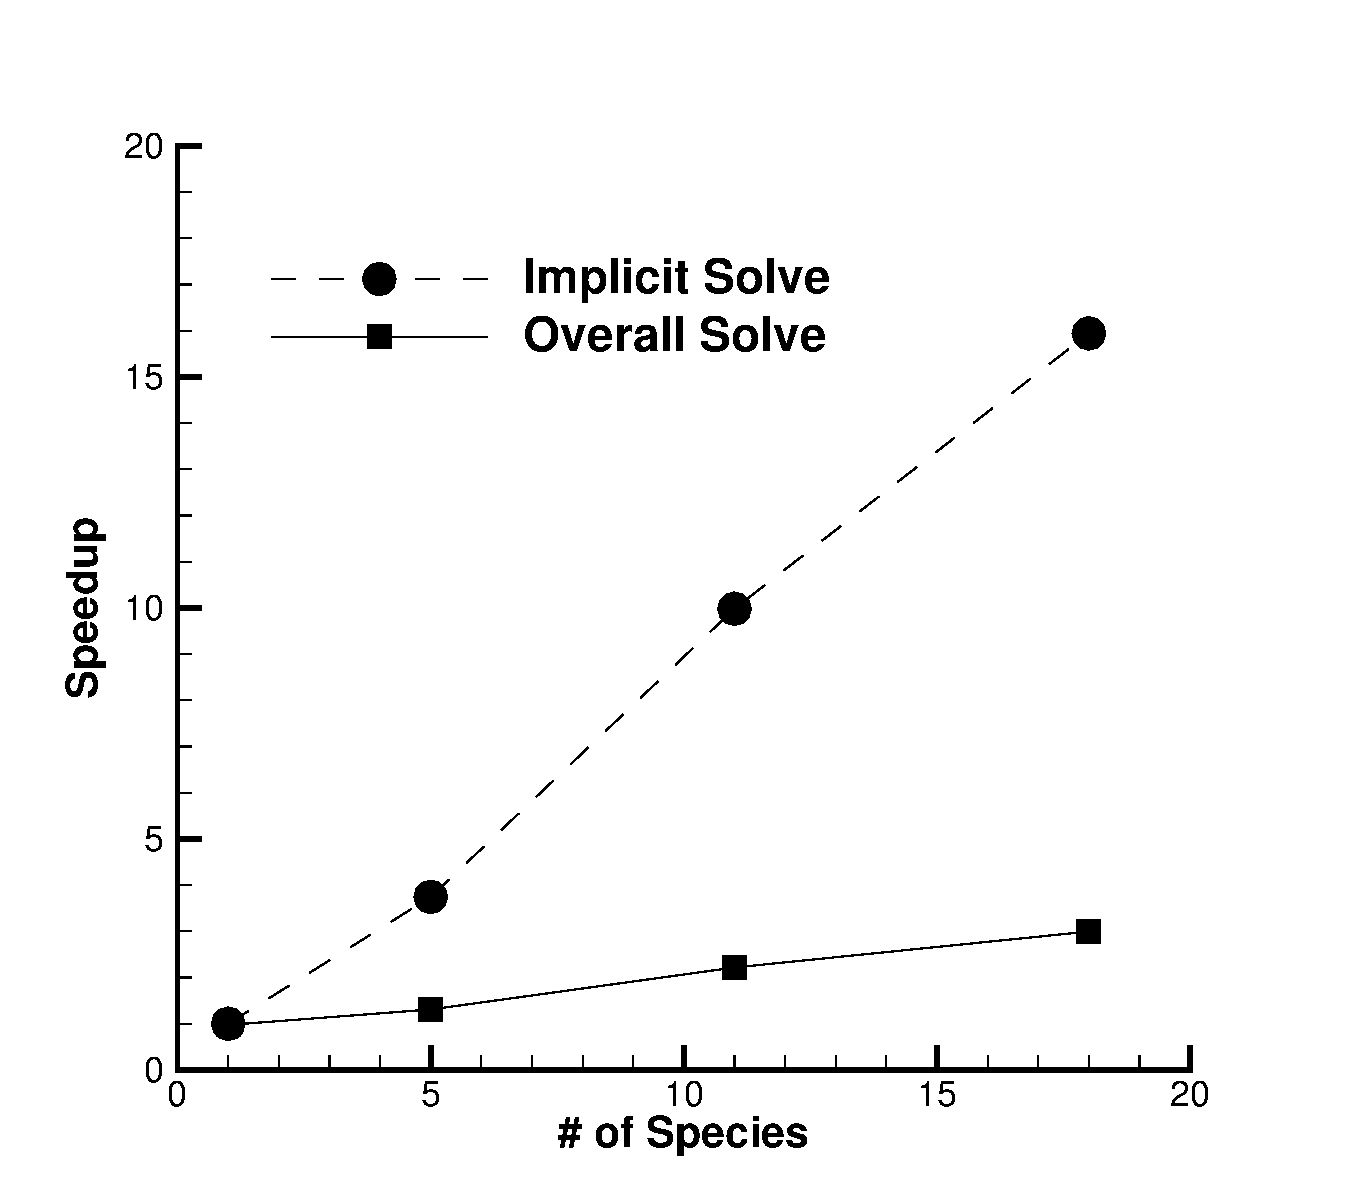
\includegraphics[width=0.45\textwidth]{figures/scitech/speedup} 
  \caption{ Relative speedup for the decoupled scheme vs. fully coupled scheme.}
  \label{rel_speedup} 
\end{figure}
%------------------------------------------------------------------------------%

\section{15 km/s Flow over Spherically-Capped Cone}

To ensure that the decoupled scheme is robust and accurate at higher velocities, both the
fully coupled and decoupled approaches were run on a sphere-cone geometry
identical to that presented by Candler et. al. \cite{candler} (10 cm nose
radius, 1.1 m length, 8$^o$ cone angle).  For this case, a simple 64$\times$64
hexahedra grid was constructed, and freestream conditions were set as
$V_{\infty} = 15000\ m/s$, $\rho_{\infty}=0.001\ kg/m^3$, $T_\infty = 200\ K$.
It was discovered that CFL limitations for the decoupled scheme were
prohibitive, because of the stiffness of the chemical source term.  In order to
converge the scheme in a manner competitive with the fully coupled approach, it
was necessary to scale the magnitude of the source term contribution to the flux
balance by a value $\omega$, such that $0 \leq \omega \leq 1$.  To ensure that
the decoupled and fully coupled approaches yielded the same result, a ramping
scheme was implemented such that no scaling was performed on the source term
when the solution was in a converged state.

\subsection{Sphere-Cone - Verification of Implementation} 

As with the cylinder test case, the surface pressure and temperature were used
as metrics to determine that both the decoupled and fully coupled approaches
give the same answer when converged to steady-state. The species composition
consisted of N, $\text{N}_2$, O, $\text{O}_2$, NO, N$^+$, $\text{N}_2^+$, O$^+$,
$\text{O}_2^+$, NO$^+$, and electrons, with 22 possible reactions. Figure
\ref{cone_predictions} shows that both methods again yield similar results, and
the high stagnation temperature indicates that this is an inviscid,
one-temperature simulation.  This demonstrates that the decoupled approach is
able to converge to the same solution as the fully coupled solution, in spite of
the chemical reactions proceeding very rapidly due to a high stagnation
temperature.

%------------------------------------------------------------------------------%
\begin{figure}
	\centering
	\begin{subfigure}[b]{0.4\textwidth}
		\centering
		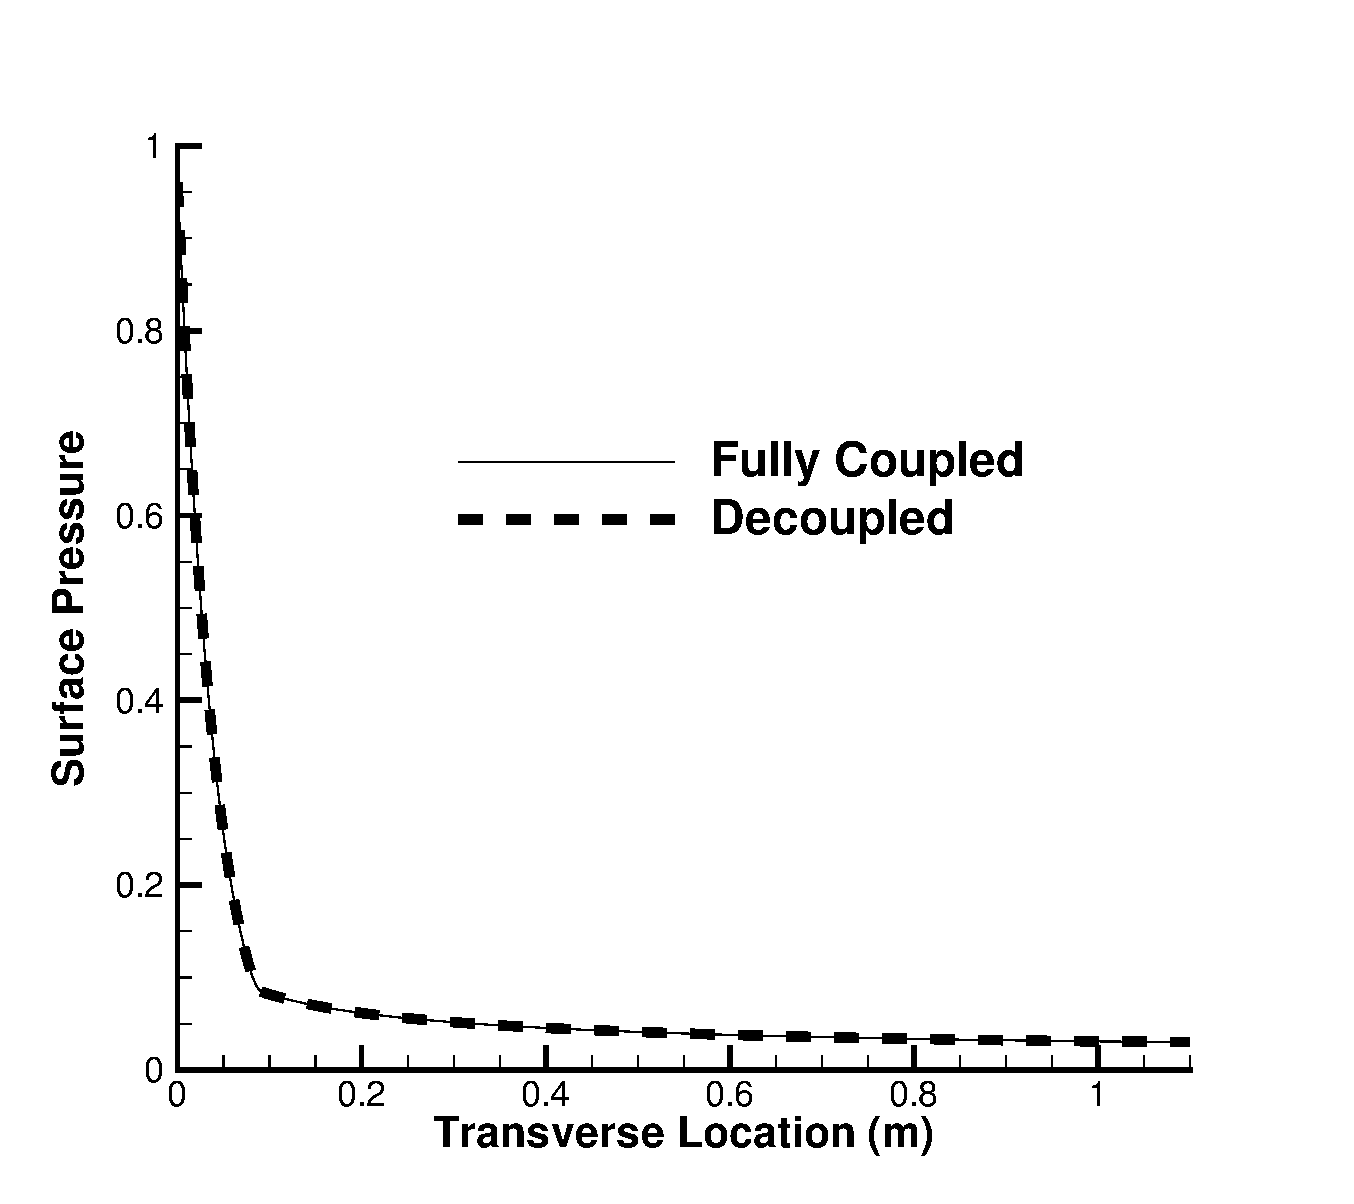
\includegraphics[width=\textwidth]{figures/scitech/surface_pressure_cone}
		\caption{Surface pressure}
		\label{cone_pressure}
	\end{subfigure}
	\begin{subfigure}[b]{0.4\textwidth}
		\centering
		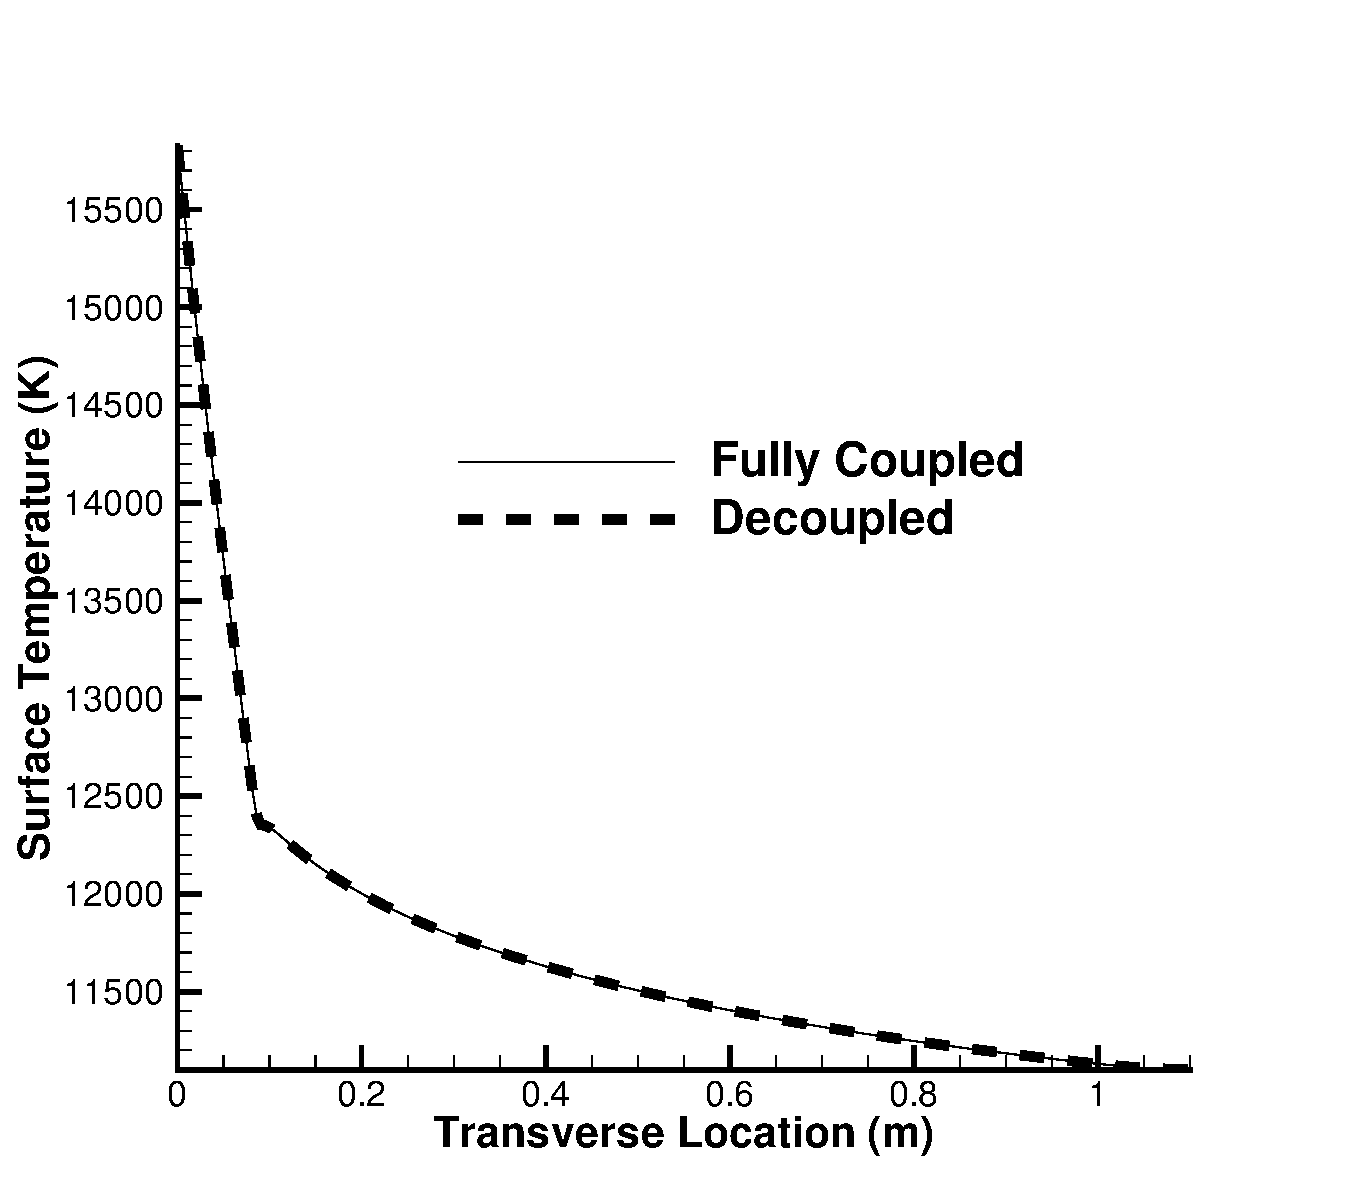
\includegraphics[width=\textwidth]{figures/scitech/surface_temperature_cone}
		\caption{Surface temperature}
		\label{cone_temp}
	\end{subfigure}
  \caption{ Sphere-cone predicted quantities. }
  \label{cone_predictions}
\end{figure}
%------------------------------------------------------------------------------%

\subsection{Sphere-Cone - Convergence Quality}

The limits on the stability of the decoupled scheme derives from introducing
explicitness in creating and destroying species.  By scaling the magnitude of
the chemical source term during the transient phase of the solve, this
instability can be mitigated, and the convergence of decoupled scheme approaches
that of the fully coupled scheme. Scaling of chemical source term was done
identically between the decoupled and fully coupled scheme by ramping the
factor $\omega$ from 0.001 to 1.0 over the first 500 timesteps. Figure
\ref{cone_convergence} shows that the convergence of both schemes progresses
nearly identically, with the decoupled scheme converging in significantly less
computational time and, interestingly, fewer timesteps.
%------------------------------------------------------------------------------%
\begin{figure}
	\centering
	\begin{subfigure}[b]{0.4\textwidth}
		\centering
    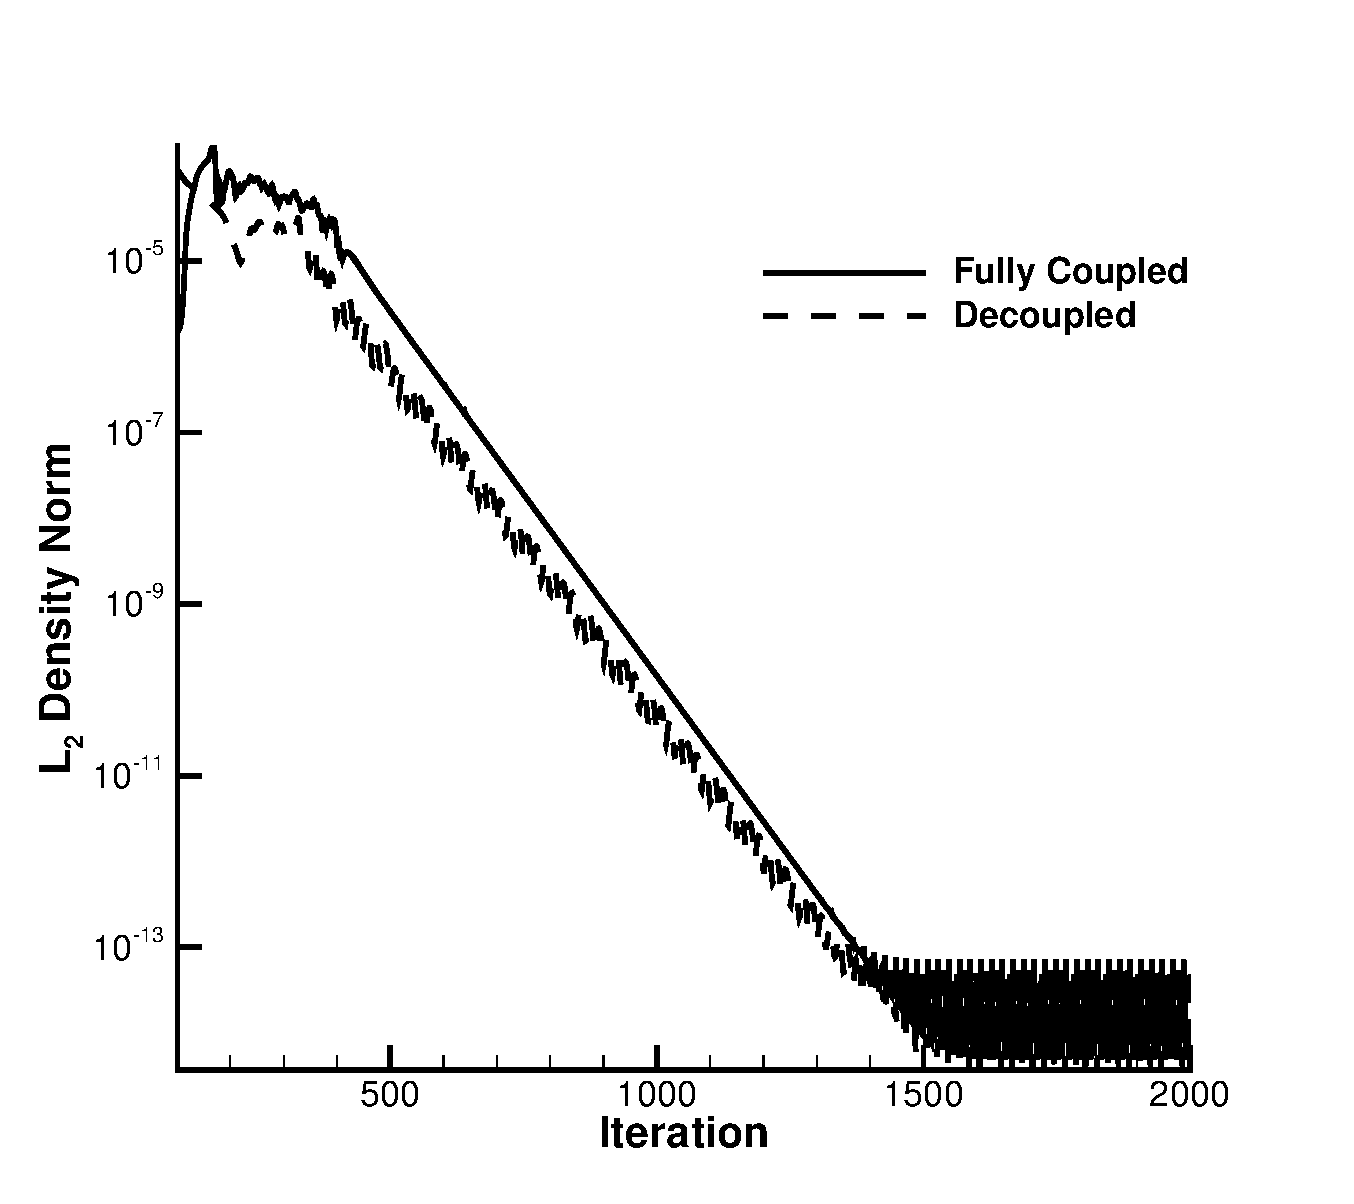
\includegraphics[width=\textwidth]{figures/scitech/cone_iteration}
		\caption{Iterations to convergence}
		\label{cone_iterations}
	\end{subfigure}
	\begin{subfigure}[b]{0.4\textwidth}
		\centering
		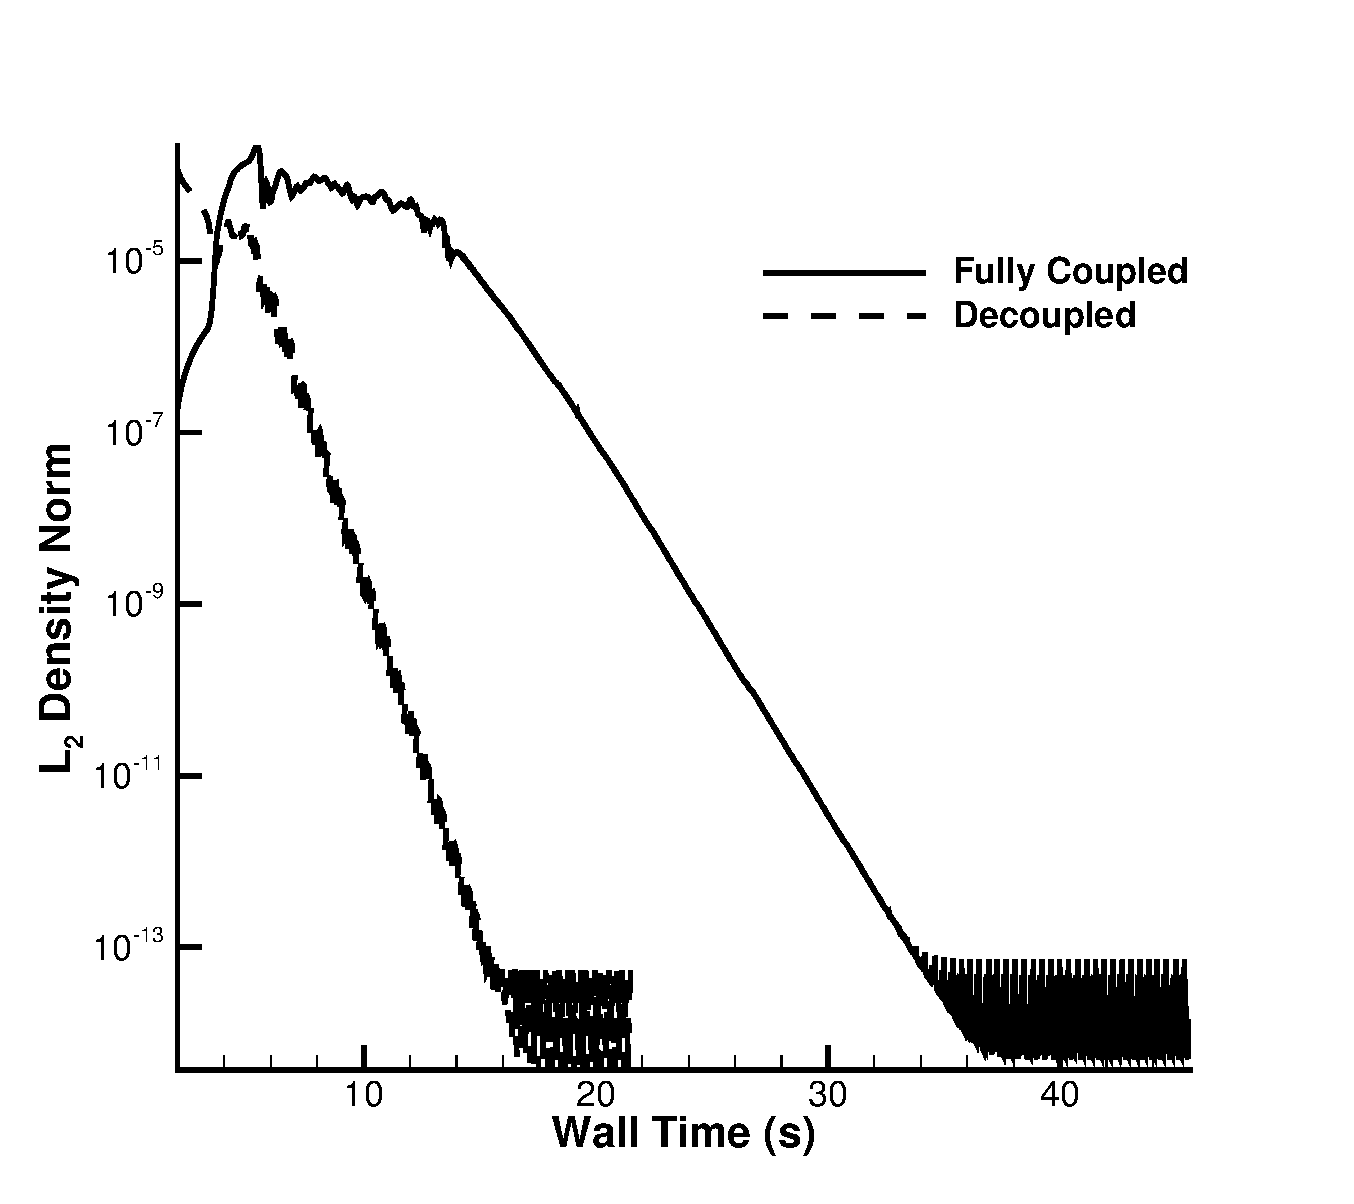
\includegraphics[width=\textwidth]{figures/scitech/cone_walltime}
    \caption{Computational time to convergence}
		\label{cone_walltime}
	\end{subfigure}
  \caption{ Sphere-cone convergence details. }
  \label{cone_convergence}
\end{figure}
%------------------------------------------------------------------------------%
This demonstrates that the decoupled scheme has significant potential to
improve the efficiency of high-velocity simulations, and that the stiffness of
the source term can be overcome in the presence of large chemical reaction
rates.

